%-------------------------- PREÁMBULO ---------------------------------------
\documentclass[letterpaper]{article}
\usepackage[utf8]{inputenc}
\usepackage[top=2cm, bottom=2cm, left=2.5cm, right=2.5cm]{geometry}
\usepackage[spanish]{babel}
\usepackage{graphicx} %Paquete para las figuras (inserción simple)
\usepackage{wrapfig} %Para ocupar el entorno wrapfigure
\usepackage{subcaption} %Para poder trabajr con subfiguras


\author{Ana Laura Reynoso \\ analaura.proteco@gmail.com}
\title{Imágenes }
\date{\today}

\begin{document}
	\maketitle
%----------------------- Inseción simple ------------------------------------
	\section{Inserción simple}
	
	\subsection{Ejemplo 1}
	\begin{flushright}
		\includegraphics[width=200pt]{assets/img1.jpg} %ancho de 200 punto
	\end{flushright}
	
	\subsection{Ejemplo 2}
	\includegraphics[height=100pt]{assets/img1.jpg} %altura de 100 punto 
	
	\subsection{Ejemplo 3}
	\includegraphics[angle=-90, width=100pt]{assets/img4}
	
	\subsection{Ejemplo 4}
	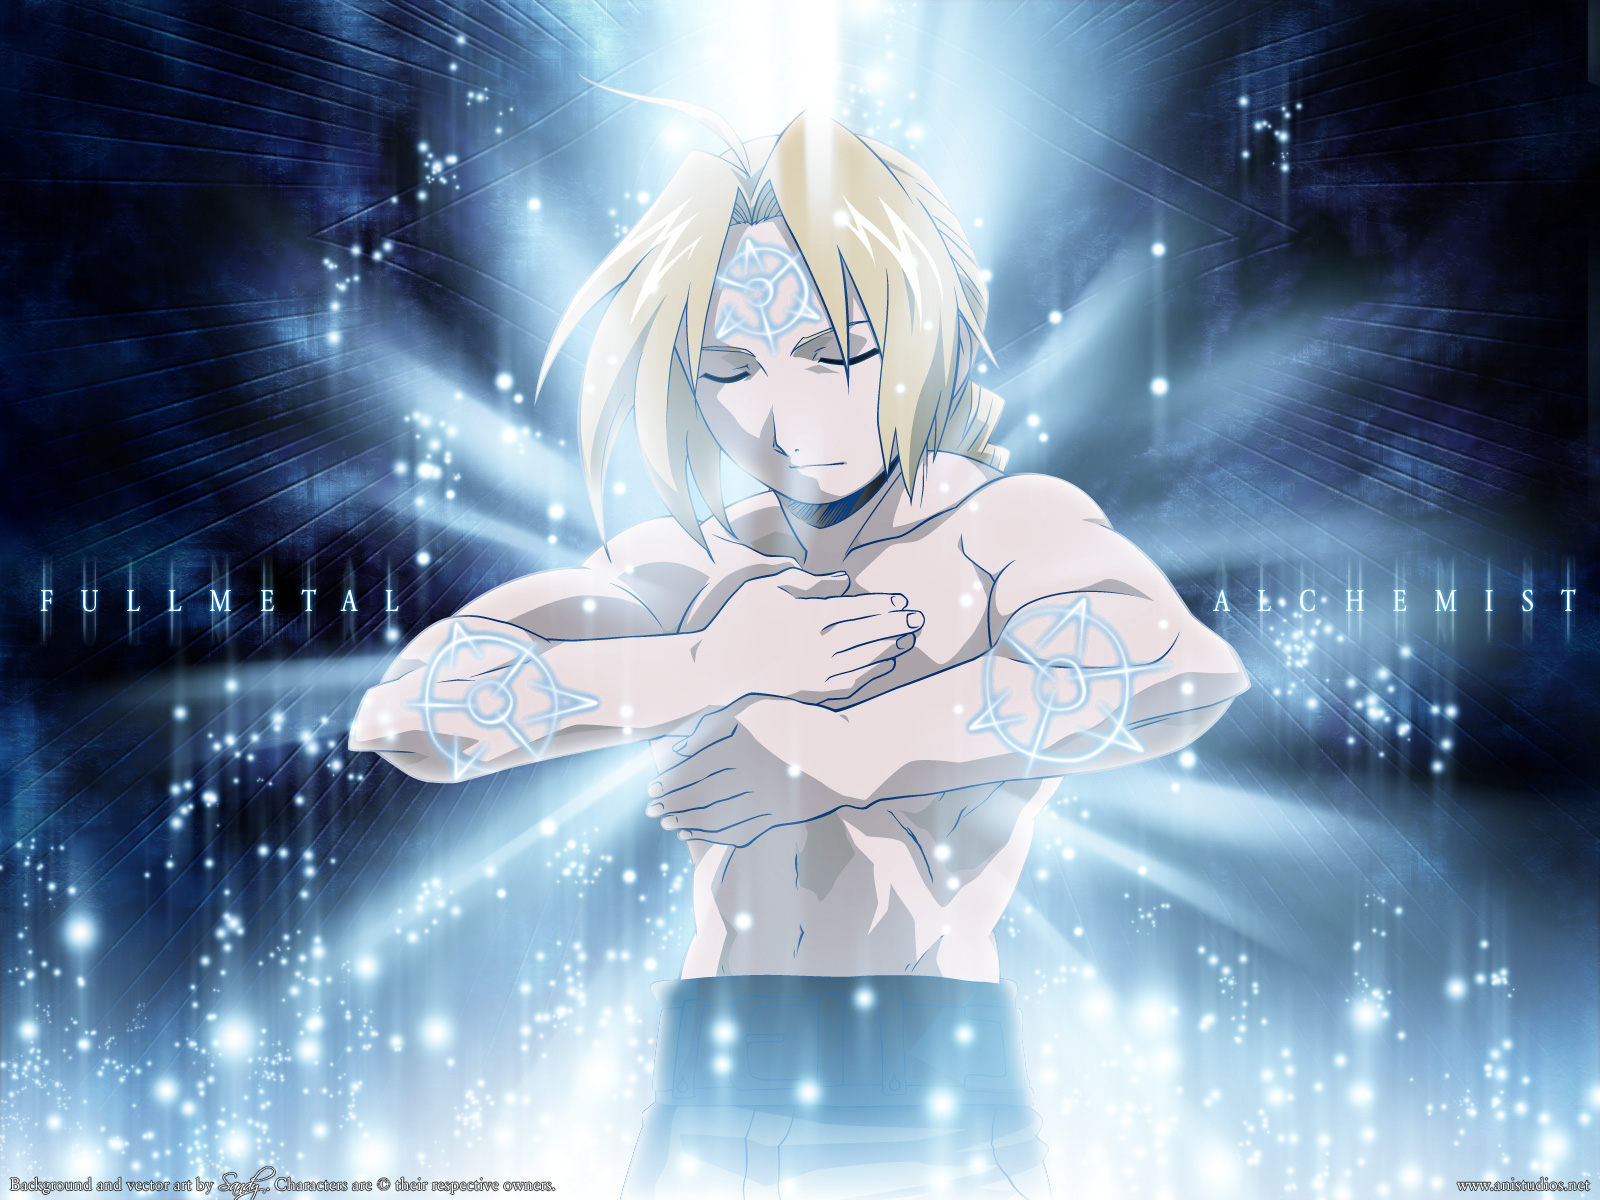
\includegraphics[scale=0.2]{assets/img7}
	
%-------------------------------- ENTORNO FIGURE ----------------------------
	\newpage
	\section{Entorno figure}
	\subsection{Ejemplo 1}
	
	\begin{figure}[h]
		\centering
		\caption{Con entorno figure}
		
\includegraphics[width=100pt]{assets/img3_2}
	\end{figure}
	
	\subsection{Ejemplo 2}	
	\begin{figure}[h]
		\centering
		\includegraphics[width=10cm]{assets/img5}
		\caption{Con entorno figure}
	\end{figure}
	
%----------------------------- ENTORNO WRAPFIGURE --------------------------
	\newpage
	\section{Entorno wrapfigure}
	
	\subsection{Ejemplo 1}
  \subsection*{Sobre encontrarse a la chica 100\% perfecta una bella mañana de
  abril}
	
  Una bella mañana de abril, en una callecita lateral del elegante barrio de
  Harajuku en Tokio, me crucé con la chica 100\% perfecta. \\
	
  A decir verdad, no era tan guapa. No sobresalía de ninguna manera. Su ropa no
  era nada especial. En la nuca su cabello tenía las marcas de recién haber
  despertado. Tampoco era joven –debía andar alrededor de los treinta, ni si
  quiera cerca de lo que comúnmente se considera una “chica”. Aún así, a quince
  metros sé que ella es la chica 100\% perfecta para mí. Desde el momento que la
  vi algo retumbó en mi pecho y mi boca quedó seca como un desierto. Quizá tú
  tienes tu propio tipo de chica favorita: digamos, las de tobillos delgados, o
  grandes ojos, o delicados dedos, o sin tener una buena razón te enloquecen las
  chicas que se toman su tiempo en terminar su merienda. Yo tengo mis propias
  preferencias, por supuesto. A veces en un restaurante me descubro mirando a la
  chica de la mesa de al lado porque me gusta la forma de su nariz.
	
	\begin{wrapfigure}{r}{0.4\textwidth}
		\centering
		\includegraphics[width=0.4\textwidth]{assets/img5}
		\caption{Alineado a la izquierda}
	\end{wrapfigure}

Pero nadie puede asegurar que su chica 100\% perfecta corresponde a un tipo
preconcebido. Por mucho que me gusten las narices, no puedo recordar la forma de
la de ella –ni siquiera si tenía una. Todo lo que puedo recordar de forma segura
es que no era una gran belleza. Extraño.

Ojalá hubiera hablado con ella. Media hora sería suficiente: sólo para
preguntarle acerca de ella misma, contarle algo acerca de mí, y –lo que
realmente me gustaría hacer– explicarle las complejidades del destino que nos
llevaron a cruzarnos uno con el otro en esa calle en Harajuku en una bella
mañana de abril de 1981. Algo que seguro nos llenaría de tibios secretos, como
un antiguo reloj construido cuando la paz reinaba en el mundo.

Después de hablar, almorzaríamos en algún lugar, quizá veríamos una película de
Woody Allen, entrar en el bar de un hotel para tomar unos cócteles. Con un poco
de suerte, terminaríamos en la cama.

	\subsection{Ejemplo 2}
	\begin{wrapfigure}{l}{0.4\textwidth}
		\centering
		
\includegraphics[width=200pt]{assets/img6}
		\caption{Alineado a la derecha}
	\end{wrapfigure}
	
  No, no se lo creería. Aunque lo dijera es posible que no quisiera hablar
  conmigo. Perdóname, podría decir, es posible que yo sea la chica 100\%
  perfecta para ti, pero tú no eres el chico 100\% perfecto para mí. Podría
  suceder, y de encontrarme en esa situación me rompería en mil pedazos, jamás
  me recuperaría del golpe, tengo treinta y dos años, y de eso se trata madurar.
  \\

Pasamos frente a una florería. Un tibio airecito toca mi piel. La acera está
húmeda y percibo el olor de las rosas. No puedo hablar con ella. Ella trae un
suéter blanco y en su mano derecha estruja un sobre blanco con una sola
estampilla. Así que ella le ha escrito una carta a alguien, a juzgar por su
mirada adormecida quizá pasó toda la noche escribiendo. El sobre puede guardar
todos sus secretos. \\

Doy algunas zancadas y giro: ella se pierde en la multitud. \\

Ahora, por supuesto, sé exactamente qué tendría que haberle dicho. Tendría que
haber sido un largo discurso, pienso, demasiado tarde como para decirlo ahora.
Se me ocurren las ideas cuando ya no son prácticas. \\

%------------------------------- SUBFIGURAS -------------------------------.

	\section{Subfiguras}
	\subsection{Ejemplo 1}
	
	\begin{figure}[h]
		\centering
		\begin{subfigure}{6cm}
			\includegraphics[width=5cm]{assets/img2}
			\caption{Mi Wero}
		\end{subfigure}
		\begin{subfigure}{6cm}
			\includegraphics[width=6.5cm]{assets/img5}
			\caption{Mi Wero y mi Negri}
		\end{subfigure}
		\caption{Ejemplo de subfiguras}
	\end{figure}


	
\end{document}
